\chapter{Literature Survey}
The literature for this project can be divided mainly into four parts. The spatial data and spatial web services on which the framework is developed. Crawling: How to find that data. Catalog Service: Once the data is found, how to store that data. How to make data easily accessible to others. And at the last Query orchestration: how to perform simple queries on the available data.

\section{Spatial Data \& Spatial Web Services}
\par
The term Geo comes from geography. Geography stores all the information of location and shape of the object in the spatial data. Spatial data stores the relationships between these data. It can also be easily mapped to a map. Spatial data is stored as raster data or vector data. Geo-server provides various kinds of functionality to this type of data. Spatial data is the data that can be mapped.Spatial data is collection of spatial object that has topology and co-ordinates. Spatial data gives geographical and shape related attributes of the data.Geographical information system is used to retrieve and operate on spatial data. Different operations can be add, visualize, annotate etc. A Geographical Information System provides various extended operation on spatial data. Different examples of such software that offers spatial services are ESRI, Microsoft SQL Server, ERDAS imagine etc.

\subsection{Classification of Spatial Data}
Open Geo-spatial Consortium(OGC) defines  Different types of object under the class geometry are as below. All the major Geo-spatial service providers and vendors provide this kind classification.The primitive four data types in spatial data are point, curve, surface and GeomCollection. Figure \ref{cosd} shows hierarchy in classification of spatial data.\\
\newline
\begin{figure}[h]
    \centering
    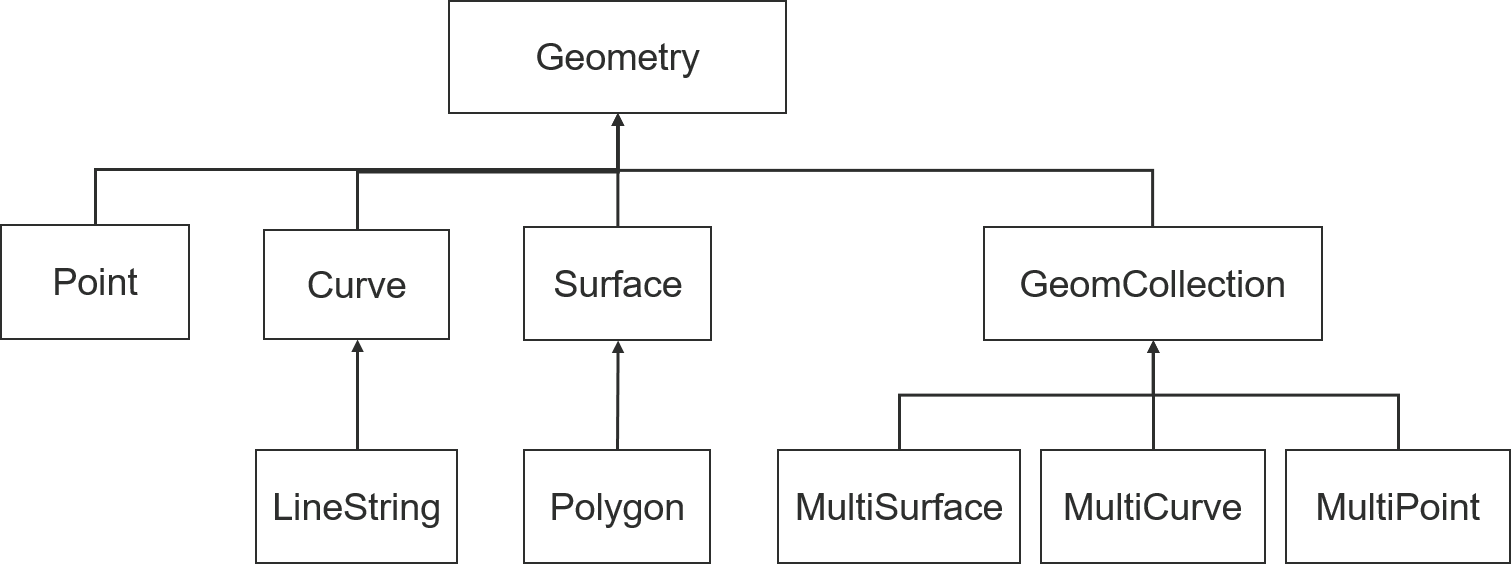
\includegraphics[width=\textwidth]{pix/p}
    \caption{Classification of spatial data}
    \label{cosd}
\end{figure}
\newline
\begin{itemize}
\item \textbf{Point}\\
Point in a map is denoted by (x, y) co-ordinates. When we see kharagpur city on a scale
of India it will be seen as a point. Point can be used to denote various objects like origin,
city, end point, top of the mountain etc. It denotes a single point consisting of longitude and latitude.\\

\item \textbf{Curve}\\
Curve is used to denote collection of points. This can be a straight line or curve. For
example, a road network can be represented with the help of line strings. Similarly, a
river can be denoted as a curve. Curve can be made with help of two distinct points.\\

\item \textbf{Surface}\\
A surface is representation of an area or a polygon. When kharagpur is seen in the scale
of west Bengal it is seen as surface or polygon. Polygon can be made using at least three non-linear points. Every polygon has a feature called boundary.\\

\item \textbf{GeomCollection}\\
Collection of basic building blocks defining a new type of geometry can be defined
with the help of GeomCollection. GeomCollection is made with combining two or more geometry types.\\

\end{itemize}


\subsection{OGC Web Services}
Open Geospatial Consortium (OGC) is the worldwide standardization body for geospatial standards. OGC provides a standardized way of accessing this geospatial data. OGC mainly provides three kinds of web services.\\
\begin{itemize}
\item \textbf{Web Map Service (WMS)}\\
Web Map service defines a way of accessing geospatial information across all geo servers in a
standard format as image. This image can be raster image or a vector image. Raster images are
of type jpg, png or bmp. Vector images contains svg format extension images. It also provides
a way to access metadata about the available information of the layers. This information can
contain type and no of layers. \\
Some of the well-defined operations in this layer are
GetCapabilities, GetMap and DescribeLayer. GetCapabilities operation returns capabilities of the server for example, what kind of services the server offers. This operation may be useful to check if a server is geo server or not by examining the kind of services it offers. GetMap service returns map images for the queried data. multiple such layer of images can be queried and then can be overlaid on top of each other. for example satellite view, terrain view, traffic view etc. Each of this layer gives additional information to the map. DescribeLayer operation describes what are the available layers and what is the metadata about the layers.\\
\item \textbf{Web Feature Service (WFS)}\\
WFS allows direct access to features contained in the map. WFS uses SOAP based interface. SOAP is used to minimize the overhead into the communication and verify cross platform stability.
For exchanging data between client and server WFS uses Geographical mark-up language(GML)
which is based on XML. Some well-defined operations in WFS are query or get feature, which
returns the feature stored on the server. We can add the feature in the repository by add feature.
We can delete feature by delete feature. Also we can update feature stored in the repository by
update feature. We can also lock certain feature to disallow modification of it while sharing via lock feature. Locked resources and features wont be accessible to change to other clients. Example of feature are the objects in the map like building or petrol pump.\\
\item \textbf{Web Coverage Service (WCS)}\\
WCS offers multi-dimensional coverage of the geo spatial data.It can provide originally retrieved data or provide processed data. It provides spatio-temporal
context to the given geographical data. For example, it can show the flow of the river changing
over the span of years. Thus we can say that WCS provides richer coverage of spatial data than
WFS or WMS. Coverage data is mainly used for scientific calculations.
\end{itemize}
\section{Spatial Web Crawler}
Spatial web crawler is a topical crawler which finds geospatial capable servers and services from the web. Sonal Patil\cite{l1} provides the base architectural guidelines for building spatial web crawler. Wenwen Li\cite{l2} says that if a server is offering geo-spatial capabilities then it can be either of the WMS, WFS or WCS server. The geo-servers must comply to OGC standards for geospatial data. This can be checked using GetCapabilities service request. We can check whether a given server offers WMS offerings or not can be checked using special suffix string added to the URL of a geo-server. More details are covered in the geo-spatial crawler part below. If the server is indeed a WMS server, It replies with and XML files containing all the data and operations it can offer. We call this as services.xml file. Once We know that the server is a geoserver many kinds of operations can be performed on it. WMS geoserver offer various operations such as GetMap, DescribeLayer, GetCapabilities etc. WMS capabilities file contains all these operations mentioned above. This is to check if a particular server is geoserver or not. If we want to crawl through the open web, then we must repeat this process. For this purpose standard operation of crawlers are performed. We maintain a buffer of frontiers which divides the boundaries of crawled web and open un-crawled web. Wenwen Li\cite{l2} also suggests to make a auto updating crawler to periodically check whether there is any addition or removal or geoserver from the existing available data. This geoserver(s) also add new data to them and remove obsolete data from the data store. Automatic updates allows this operations to be done periodically and maintain the overall consistency of the data.\\
\par
Marc Najork\cite{l3} suggests that the task of crawling the web for WMS servers can be done parallel. He suggests to use parallel FIFO queues to carry out the operation efficiently. To check whether the URL already exists or not in the crawled set, he suggests to use efficient data structures to check set membership such as HashSet. He also suggests to use priority in crawling based on various methods such as PageRank.\\
\par
Lopez-Pellicer\cite{l9} suggests that there might be already available geoservers and catalog services on the web. We must efficiently identify this catalog services to different type of OGC compliant services. So that different kind of queries can be forwarded to different geo servers or catalog services. Dirk Ahlers\cite{l4} suggests an architecture to crawl and parse available geoserver(s) and store the available data efficiently. They also suggests to index the data so there data can be retrieved efficiently. This methods is described as focused crawling.\\
\par
Li, W., et al.\cite{l5} suggest a method to semantically crawls the web. In his approach he maintains a hierarchy of geospatial objects to identify parent children relationship. For example, river is a type of water-body. This kind of type of relationships can be used to manage and index available data and geoservers efficiently. JIANG Jun\cite{l6} suggests similar methods for WFS servers.


\section{Catalog Service for Geo-Spatial Data}
Catalog service provides discovery and publishing of geospatial metadata information. Manoj Paul\cite{l14} provides a service oriented approach for discovery and retrieval of spatial data as web services. Nogueras et al.\cite{l15} discusses about design and storage mechanisms in a real world catalog service. 
\newline
\par In this section we will look at two types of available catalog services for geospatial data. Python catalog service for web(PyCSW)\cite{l7} offers a model architecture for implementing a OGC compliant web service catalog portal. In this model, series of module are used to invoke a hierarchy such that decomposition of the functions and use case is efficient and easy. In this architecture many of the modules can work in parallel. Important modules are crawler, WMS capabilities files, Database to store geospatial data and a server to provide interface to functions. All the functions are implemented and run via programs on a server. This wsgi server acts as a geospatial catalog which accumulates data from various other geospatial repositories and catalogs available on the open web. Using the PyCSW interface many types of applications can be invoked. PyCSW provides various APIs for OGC compliant operations. For example, using GetMap a user or application can get all the data from all the crawled repositories in a single place. We can know the information available for the layers and from where this information is available. The detailed implementation of this architecture is discussed in the later chapters.\\
\par
GeoServer\cite{l10} also offers such services but it also offers powerful management tools and admin console to function via graphical user interface. It provides services to work with various data formats such as shape files or GML format, it supports various database options for storage purpose and it is extensible to add more services. In our approach, we will mainly use GeoServer as our catalog service. However it should be noted that GeoServer is more resource intensive than PyCSW as it provides more services than the latter. It provides integration with various programming languages like Python, Java, Ruby and PHP.
\section{Query Orchestration}
Query Orchestration provides query operations on the spatial data from the database. Various operations are available as OGC standards to operate and query on the data. Query orchestration also deals with indexing and ranking. Here we have used Quad tree for indexing spatial data. Quad tree\cite{l13} is particularly standard data structure for indexing spatial data. Another interesting concept is ranking by quality preferences\cite{l11}. In this concept we take the cumulative property of spatial neighbourhood to calculate ranking for the spatial objects. Ranking data by quality preferences is a advanced method and requires extra information about quality of data.\\
\par
Once the catalog service is built it can directly act as a single point for querying multiple repositories. The catalog server in-fact acts as a mediator while getting the queried data from other repositories. Different type of example queries are listed below.

\begin{itemize}
\item \textbf{Service metadata information}\\
Describes what kind of OGC compliant web services are offered by the catalog server or geo-server.
\item \textbf{GetLayers}\\
An interface can be built to provide information about list of available layers.
\item \textbf{GetOperations}\\
List of available operations can be provided that gives the information about the list of operations that are offered by the geoserver or catalog service.
\item \textbf{GetBoundingBox}\\
We can get the information about the bounding box of the layers or map that covers the total area.
\item \textbf{GetMap}\\
The map of particular layer can be retrieved.
\item \textbf{DrawMap}\\
The map of particular layer/data can be retrieved and placed onto another map. This is useful to find area of interest in the particular map by superimposing the queried data to generic map.

\end{itemize}